%************************************************
\chapter{Random Search Strategies}\label{ch:randomSearchStrategies}
%************************************************
The term \emph{search problem} has been mentioned several times throughout the preceding chapters, but what does it actually describe? A very simple and intuitive form requires a searcher -- such as a human, an animal, an organism, or any kind of particle or abstract object, which is able to move and explore the search realm -- and at least one target.

Even though this seems to be a very basic problem to which most likely everyone can relate (``Where are those keys again!'') it occurs in many fields, at all scales, and can take very complex forms. Examples range from the hunt for hostile submarines during World War II, castaway rescue operations, the recovery of an atomic bomb in the Mediterranean Sea near Palomares in 1966, and the rescue of the lost nuclear submarine Scorpion near the Azores in 1968, over animals searching for food, mates, or shelter and microorganisms (see \autoref{ch:activeMotion}), to chemical reactions and genomic transcription \cite{benichou:2011}.

Despite the diversity of all these different search problems they have one more thing in common: the \textit{search time} -- the time it takes the searcher to find the target -- is a limiting factor. The consequences of long search times depend on the situation and are as diverse as the search problems themselves. They can range from just being annoying, as in the case of being late due to the search for keys, to being crucial in living or dying, if \eg the search burns more energy than the target food can provide, which will eventually lead to starvation and end in death. Therefore, the minimization of the search time is an essential and non-trivial task in most cases.

\section{Classification of search strategies}\label{sec:class-search-strategies}
Naturally, evolution has yielded many different \textit{search strategies} as efficient species were able to surpass their rivals and thus evade extinction. Also there is abundant scientific and academic interest in search strategies, which has led to the categorization of search strategies into \textit{systematic} versus \textit{random} search.

Systematic search requires the searcher to be able to keep at least a short memory of its past explorations in the search domain. Humans, for instance, are able to draw a (mental) map of the surrounding space and thus perform highly systematic searches (see \autoref{fig:systematicSearchPatterns}). On the other hand, a searcher with very low or no spatial memory at all has no choice but to follow a random trajectory.

In the latter case, the random walk theory introduced in \autoref{ch:modelingActiveMatter} provides powerful tools for the modeling and analysis of such search processes.

\begin{figure}[bth]
 \myfloatalign
 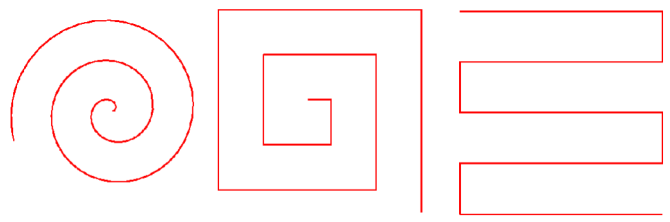
\includegraphics[width=0.8\linewidth]{gfx/systematicSearchPatterns}
 \caption[Patterns of systematic search]{Examples of patterns for systematic exploration of space -- from left to right: spiral, expanding square, lawn-mower \cite{benichou:2011}.}\label{fig:systematicSearchPatterns}
\end{figure}

Additionally, one can distinguish between search with or without cues. Although the target is usually hidden, in practical cases there are often cues in the environment that provide the searcher with information of the whereabouts. Such information can be provided by \eg odor, sounds, and chemical concentrations or gradients. In this work, we focus on random search problems with and without cues.

\section{First-passage properties}
The search time is a limiting quantity in random search problems and thus it is essential to use search strategies which minimize it. In this work, we quantitatively measure and compare the efficiency of different strategies based solely on their search time, even though there are other measures available such as \eg energy expenditure or risk factors.  For this purpose, the \textit{first-passage} theory provides adequate tools.

Especially in the context of random walks there is a vast literature available on first-passage phenomena. \graffito{In first-passage problems we are not interested in how trajectories look like but rather when a specific point is reached for the first time.}There, the fundamental issue is to determine the time dependence of the \textit{first-passage probability} $\F(\bv{x},t)$. This is the probability that at time $t$ a random walk hits $\bv{x}$ for the very first time. Note that we are \emph{not} concerned with explicit forms of trajectories of walks.

Another fundamental and related issue is to evaluate the \textit{first-passage time $\tau$}. This is the time it takes the random walker to reach a specified location $\tarv$ for the first time. Or in a more precise way: given a fixed starting location $\bv{x_0}$, how long does it take for the walker to reach the specified location $\tarv$ for the first time \emph{on average}. This quantity is called the \acfi{mfpt}\acused{mfpt}. Consequently, the \ac{mfpt} $\mfpt$ corresponds to the average search time in an ensemble of similar problems with the same initial and boundary conditions.

Prior to the question of the mean time required to reach a certain target destination, however, we can also ask for the \textit{hitting probability} (sometimes \textit{exit probability}). That is the probability of hitting $\tarv$ given enough time ($t\rightarrow\infty$). In particular one can show that under certain conditions the hitting probability can be zero, meaning that the walker will never reach its target and thus making the question for the \ac{mfpt} trivially irrelevant.

As a last remark, before moving onto actual first-passage problems, we want to emphasize that first-passage phenomena are not limited to spatial problems, although the text and the terminology around search problems may lead to a different perception. The vector $\tarv$ may represent not only locations but any abstract object or value for which it is interesting to know when it reaches a certain threshold for the first time. Some practical examples are the value of stocks or market prices, the firing of neurons in the brain \cite{amit:1989}, and the evolution of the number of individuals in a population.

In the following, we will start with a basic and simple first-passage problem to get acquainted with first-passage properties. Afterwards, we will introduce a few general approaches that are applicable to more complex problems.

\subsection{An intuitive approach to first-passage properties}\label{ssec:intApproach}
To get started with first-passage properties, we will introduce a very simple first-passage problem for which we will derive the hitting probability and the \ac{mfpt} in a straightforward and intuitive way.

Let us consider the \ac{srw} on a one-dimensional lattice as introduced in \autoref{sec:SIRW}. Starting from the origin $n=0$ at time $m=0$, we are interested in the probability of reaching site $n=2$ before \mbox{$n=-2$}. In order to answer this question, it is convenient to calculate the probability for any starting position $n_0\in\left[-2,2\right]\subset\Z$ in a set of coupled equations. Of course, the desired probability would be $1$ ($0$) if $2 < n_0$ ($n_0 < -2$). We introduce the hitting probability $q_i$ for $i\in\left[-2,2\right]\subset\Z$ as follows:
\begin{center}
 $q_i \quad \equiv$ \quad probability of visiting site $n=2$ before $n=-2$ starting from $n_0=i$.
\end{center}
With this, one can write the set of coupled equations by shifting the problem of obtaining the probability $q_i$ to the problem of obtaining the probabilities of the neighboring sites $q_{i-1}$ and $q_{i+1}$ for all inner sites $i \in \left\{-1,0,1\right\}$. Together with the boundary conditions $q_{-2}=0$ and $q_2=1$ one can then easily derive the solution:
\begin{equation*}
 \left\{\quad
 \begin{aligned}
  q_{-2} &= 0
  \\
  q_{-1} &= \frac{1}{2}q_{-2}+\frac{1}{2}q_{0}
  \\
  q_{0} &= \frac{1}{2}q_{-1}+\frac{1}{2}q_{1}
  \\
  q_{1} &= \frac{1}{2}q_{0}+\frac{1}{2}q_{2}
  \\
  q_{2} &= 1  
 \end{aligned}
 \quad
 \right\} \quad \xlongrightarrow[\textrm{equations}]{\textrm{solve}} \quad \left\{\quad
 \begin{aligned}
  q_{-2} &= 0
  \\
  q_{-1} &= \frac{1}{4}
  \\
  q_{0} &= \frac{1}{2}
  \\
  q_{1} &= \frac{3}{4}
  \\
  q_{2} &= 1
 \end{aligned}
 \quad
 \right\}.
\end{equation*}
Analogously, one can derive the \acp{mfpt} -- which on the lattice are equivalent to the number of steps -- for the different starting positions by introducing
\begin{center}
 $\mfpt_i \quad \equiv$ \quad \ac{mfpt} for visiting site $n=2$ starting from $n_0=i$,
\end{center}
and assuming that the left boundary at $n=-2$ is reflective\graffito{\textbf{Note:} If the left boundary at $n=-2$ is absorbing, meaning that it will capture the walker and keep it for all times, the \acp{mfpt} for all starting positions become infinite because of $\mfpt_{-2}=\infty$ (except for $\mfpt_{2}=0)$.}. Then one finds:
\begin{equation*}
 \left\{\quad
 \begin{aligned}
  \mfpt_{-2} &= \mfpt_{-1}+1
  \\
  \mfpt_{-1} &= \frac{1}{2}\mfpt_{-2}+\frac{1}{2}\mfpt_{0}+1
  \\
  \mfpt_{0} &= \frac{1}{2}\mfpt_{-1}+\frac{1}{2}\mfpt_{1}+1
  \\
  \mfpt_{1} &= \frac{1}{2}\mfpt_{0}+\frac{1}{2}\mfpt_{2}+1
  \\
  \mfpt_{2} &= 0
 \end{aligned}
 \quad
 \right\} \quad \xlongrightarrow[\textrm{equations}]{\textrm{solve}} \quad \left\{\quad
 \begin{aligned}
  \mfpt_{-2} &= 16
  \\
  \mfpt_{-1} &= 15
  \\
  \mfpt_{0} &= 12
  \\
  \mfpt_{1} &= 7
  \\
  \mfpt_{2} &= 0
 \end{aligned}
 \quad
 \right\}.
\end{equation*}

As one can see, in this example the derivation of the hitting probability as well as the \ac{mfpt} is very easy. However, in most situations this intuitive approach is not useful and therefore a general framework is needed.

\subsection{Electrostatics approach}\label{ssec:electrostatics-approach}
Although the approach in \autoref{ssec:intApproach} was used for an easy and very specific problem, the generalization of this problem already leads to an interesting analogy to electrostatics, which then again yields some interesting results. Therefore, we want to be more general here and set $\Omega \subseteq \R^d$, \ie we deal with a d-dimensional continuous random walk. Note that the derivations in this section partly follow the derivations presented in the book \mycitet{krapivsky:2010}.

\subsubsection{Hitting probability}\label{sssec:hitting-prob}
In analogy to \ref{ssec:intApproach} we divide the boundary $\partial\Omega$ into two disjoint subsets $\partial\Omega_1$ and $\partial\Omega_2$. This means, $\partial\Omega_1\cup\partial\Omega_2=\partial\Omega$ and \mbox{$\partial\Omega_1\cap\partial\Omega_2=\emptyset$}. We can then ask for the hitting probability $q\bra{\bv{x}}$, $\bv{x}\in\Omega$, \ie that the random walker hits $\partial\Omega_1$ before $\partial\Omega_2$ starting from $\bv{x}$. Even though one could have more complex boundaries, this is sufficient for our purposes.

\graffito{\textbf{Note:} As a consequence of the translational invariance of the problem it is sufficient to consider the interval $\bra{0,N}$ and translate the results to any other interval.}However, firstly we go back to the one-dimensional discrete and finite case as in \ref{ssec:intApproach} and set $\Omega \subset \N$, $\Omega=\bra{0,N}$. Then, it is $\partial\Omega_1=\left\{N\right\}$, $\partial\Omega_2=\left\{0\right\}$, and $q\bra{\bv{x}} = q\bra{x} \equiv q_n$. We can then define the boundary value problem as
\begin{equation*}
 q_n =
 \begin{cases}
  \frac{1}{2}\bra{q_{n-1}+q_{n+1}}, & \textrm{if }n\in\Omega,\\
  1, & \textrm{if }n\in\partial\Omega_1,\\
  0, & \textrm{if }n\in\partial\Omega_2.
 \end{cases}
\end{equation*}
The term boundary value problem is explicitly used here as this problem corresponds to the discrete \textit{Laplace} equation. We know that the solution for this type of equation must be of the linear form $A+Bn$ and invoking the boundary conditions yields
\begin{equation*}
 q_n = \frac{n}{N}.
\end{equation*}
We can check that this result is in agreement with our findings in \autoref{ssec:intApproach}. However, so far we only generalized the problem of the simple type in \ref{ssec:intApproach}. Yet, the observation that this problem is based on solving the Laplace equation leads to the following approach.

\bigskip

\noindent We consider the d-dimensional discrete random walk with the above definitions. Taking the continuum limit, the hitting probability then satisfies the Laplace equation
\begin{equation*}
 \Laplace q\bra{\bv{x}} = 0,\quad \forall \bv{x}\in\Omega,
\end{equation*}
and together with the boundary conditions we can define the boundary value problem\graffito{\textbf{Note:} If $\partial\Omega_1$ and $\partial\Omega_2$ do not contain the entire boundary of $\Omega$, then on the remaining parts, the condition $\nabla_n q=0$ is to be met, with $\nabla_n$ the normal derivative.}
\begin{equation}\label{eq:bvp-hittingprob}
 \begin{cases}
  \hfill\Laplace q\bra{\bv{x}} = 0, & \forall \bv{x}\in\Omega,\\
  \hfill q\bra{\bv{x}} = 1, & \forall \bv{x}\in\partial\Omega_1,\\
  \hfill q\bra{\bv{x}} = 0, & \forall \bv{x}\in\partial\Omega_2,
 \end{cases}
\end{equation}
which is equivalent to the boundary value problem for the electrostatic potential. Therefore, all known results from electrostatics can be used to deduce results for the hitting probability $q(\bv{x})$ in arbitrary domains $\Omega$.

As an example, consider a random walker in $\R^d$ (see \autoref{fig:hyperspheres-sketch}) at a distance $x = \norm{\bv{x}}_2$ from the origin, with $\norm{\cdots}_2$ denoting the \textit{Euclidean} norm in $\R^d$. The walker is located between two hyperspheres of radius $R<x\ll R_\infty$, \ie the domain \mbox{$\Omega = [\R^d - \B_R^d(0)] \cap \B_{R_\infty}^d(0)$}, where $\B_R^d(\bv{x_0})$ is the d-dimensional hypersphere with radius $R \in \R$ and center $\bv{x_0} \in \R^d$, \ie \mbox{$\B_R^d(\bv{x_0}) = \{\bv{r} \in \R^d; \norm{\bv{r}-\bv{x_0}}_2 \leq R\}$}. Then it reads $\partial\Omega_1 = \partial\B_R^d(0)$ and $\partial\Omega_2=\partial\B_{R_\infty}^d(0)$.

\begin{figure}[bth]
 \myfloatalign
 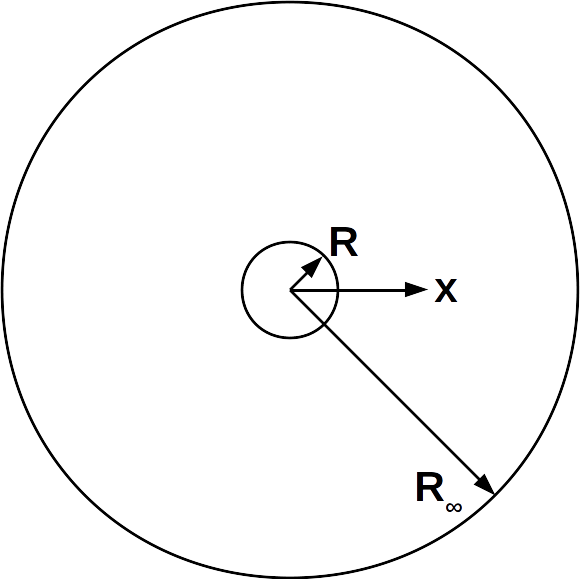
\includegraphics[width=0.4\linewidth]{gfx/hyperspheres}
 \caption[Sketch of radii relations]{Schematic sketch of the relation between the radii of the d-dimensional hyperspheres.}\label{fig:hyperspheres-sketch}
\end{figure}

For the outer sphere the index suggests that we want to take the limit $R_\infty \rightarrow \infty$ later on. Therefore, the interesting question is: what is the probability that the walker hits the inner sphere before it hits the outer sphere, namely vanishes into space. To answer this, we have to solve \autoref{eq:bvp-hittingprob} and from electrostatics we know that the result depends heavily on the dimension $d$:
\begin{description}
 \item[$d=1$:] This corresponds to the case that we have already considered. The solution is of the form $q(x) = A+Bx$. Since $q(x)$ is a probability and we take the limit $R_\infty \rightarrow \infty$, $B$ needs to be zero in order to keep $q(x) \in [0,1]$ as $x\rightarrow\infty$. The boundary condition on $\partial\Omega_1$ then leads to the trivial hitting probability $q(x)=1$ which is in contradiction to the boundary condition on $\partial\Omega_2$, however, since we take the limit $R_\infty \rightarrow \infty$ the second boundary condition becomes obsolete, \ie $\partial\Omega_2 = \emptyset$ and $\Omega = \R - \B_R^1(0)$. Let's interpret this result: the walker is moving on a one-dimensional continuous line with a boundary in one direction. The probability of eventually hitting this boundary during its walk is equal to one, no matter how far away the walker starts. Also, as a direct consequence, the walker hits the boundary infinitely often. Random walks with this property are called \textit{recurrent}.
 \item[$d=2$:] We find the solution in the theory of electrostatics again, which yields $q(\bv{x}) = q(x) = A + B \ln(x/R)$. With analogous reasoning as in the one-dimensional case we obtain $B=0$ and $A=1$. Therefore, the 2-dimensional random walk is recurrent as well.
 \item[$d\geq3$:] The solution is $q(\bv{x}) = q(x) = A + B x^{d-2}$. Here, the limit of $x \rightarrow \infty$ does not lead to divergence. By using the boundary conditions we obtain
 \begin{equation}\label{eq:hittingprobd=3}
  q\bra{x}=\frac{(R/x)^{d-2} - (R/R_\infty)^{d-2}}{1 - (R/R_\infty)^{d-2}}
 \end{equation}
 and by taking the limit
 \begin{equation}\label{eq:coulomb-formula}
  \lim\limits_{R_\infty\rightarrow\infty}{q(x)} = \bra{\frac{R}{x}}^{d-2}
 \end{equation}
 we obtain a formula which is equivalent to the Coulomb formula. We explicitly assumed a very specific shape for the hypersurface $\partial\Omega_2$, however one can heuristically explain that this result is independent of the shape of $\partial\Omega_2$ as long as the infimum of the distance of $\partial\Omega_2$ to the location of the walker (and thus to the inner sphere) is large, \ie the surface $\partial\Omega_2$ is far away from everything. By setting $R_\infty \equiv \inf\limits_{\bv{r}\in\partial\Omega_2} \norm{\bv{x}-\bv{r}}_2 \gg x$, one can always find a hypersphere ``within'' $\partial\Omega_2$ for which one can derive \autoref{eq:hittingprobd=3}. Since $R \leq x \ll R_\infty$ the terms $(R/R_\infty)^{d-2}$ become negligibly small for far away outer surfaces. Although we do not give an exact mathematical proof at this point, the essence is that for $d\geq3$ the hitting probability is given by the Coulomb formula \ref{eq:coulomb-formula} and therefore, hitting the inner sphere is not given with certainty as it was the case in lower dimensions. Such walks with nonzero probability to not hit every $\bv{x} \in \Omega$ are called \textit{transient}.
\end{description}

\bigskip

\noindent The electrostatic approach helped us to derive the interesting property that random walks are recurrent for $d \leq 2$ and transient for higher dimensions. Since we are only interested in the \ac{mfpt}, however, we hold the hitting probability in abeyance from here on and only concentrate on the \acp{mfpt}.

\subsubsection{First-passage time}
Again we consider a domain $\Omega\subseteq\R^d$ and we are interested in the average time $\mfpt \in \R_0^+$ it takes the walker to reach a certain subset $U\subset\clos{\Omega}$ for the first time. Here, we want to constrain ourselves to $U=\partial\Omega$, \ie we are interested in the time it takes the walker to hit the boundary of the domain $\Omega$.

As a first step, again we simplify and consider the one-dimensional symmetric random walk in continuous space and time with diffusion coefficient $D$. We set $\Omega = \R^+$, $\partial\Omega=\{0\}$ and the starting position of the walker $x(t=0)=x_0 \in \Omega$. From \autoref{sssec:hitting-prob} we know that this walk is recurrent and will eventually visit the origin. To find $\mfpt$ we need to take the average
\begin{equation}\label{eq:avg-of-tau}
 \mfpt \equiv \avg{\tau(x_0)} = \int\limits_0^\infty \tau \F(0, \tau \,|\, x_0) \diff \tau,
\end{equation}
thus, we need to know the first-passage probability $\F(0, \tau \,|\, x_0)$ which is the probability density of hitting the origin at time $\tau$ under the condition that the walk starts from $x_0$. In order to find $\F(0, \tau \,|\, x_0)$, we use another method from electrostatics. We first need to solve the diffusion equation \ref{eq:diffusion-equation} for the probability density $\P(x,t \,|\, x_0)$, which is the probability that the walker started from $x_0$, is at $x$ at time $t$ and has not yet reached the origin. Therefore, we use the image method and place another walker at $x=-x_0$ so that we have the initial and boundary value problem
\begin{equation*}
 \begin{cases}
  \dfrac{\partial \P(x, t \,|\, x_0)}{\partial t} = D \dfrac{\partial^2 \P(x, t \,|\, x_0)}{\partial x^2} & \textrm{if } x \in \Omega \\
  \P(x,t \,|\, x_0) = 0 & \textrm{if } x = 0 \\
  \P(x,t \,|\, x_0) = \delta(x-x_0) + \delta(x+x_0) & \textrm{if } t = 0.
 \end{cases}
\end{equation*}
The linearity of the diffusion equation allows us to quickly derive the solution with the aid of \autoref{eq:gauss-distr}
\begin{equation*}
 \P(x,t \,|\, x_0) = \frac{1}{\sqrt{4 \pi D t}}\left[e^{-(x-x_0)^2 / 4 Dt} - e^{-(x+x_0)^2 / 4 Dt}\right].
\end{equation*}
Then the first-passage probability $\F(0, \tau \,|\, x_0)$ is the flux through the origin in the time interval $(\tau, \tau+\diff \tau)$, thus
\begin{equation*}
 \F(0, \tau \,|\, x_0) = D \left. \dfrac{\partial \P}{\partial x} \right|_{x=0} = \dfrac{x_0}{\sqrt{4 \pi D \tau^3}} e^{-x_0^2 / 4 D \tau}
\end{equation*}
and we see that \autoref{eq:avg-of-tau} does not converge, \ie $\mfpt$ is infinite $\forall x_0 \in \Omega$. This means that the one-dimensional random walk in fact is recurrent and visits every $x \in \Omega$ infinitely often, however, the average time it takes to (re-)visit some $x$ is infinite.

\bigskip

\noindent Again we can derive a more general solution approach from these findings. We consider a continuous d-dimensional random walk in a finite domain $\Omega \subset \R^d$. Then we have the initial and boundary problem
\begin{equation*}
 \begin{cases}
  \dfrac{\partial \P(\bv{x}, t \,|\, \bv{x_0})}{\partial t} = D \Laplace \P(\bv{x}, t \,|\, \bv{x_0}) & \textrm{if } \bv{x} \in \Omega \\
  \P(\bv{x},t \,|\, \bv{x_0}) = 0 & \textrm{if } \bv{x} \in \partial \Omega \\
  \P(\bv{x},t \,|\, \bv{x_0}) = \delta(\bv{x}-\bv{x_0}) & \textrm{if } t = 0.
 \end{cases}
\end{equation*}
We then need to follow the same steps as in the one-dimensional case. First we need to solve the integral
\begin{equation*}
 \F(\bv{x} \in \partial \Omega, \tau \,|\, \bv{x_0}) = -D\int\limits_{\partial \Omega} \nabla \P(\bv{x}, \tau \,|\, \bv{x_0}) \diff \bv{S}
\end{equation*}
and then we need to take the average
\begin{equation*}
 \mfpt = \int\limits_0^\infty \tau \F(\bv{x} \in \partial \Omega, \tau \,|\, \bv{x_0}) \diff \tau.
\end{equation*}
However, this procedure requires a decent amount of work and if we are only interested in the \ac{mfpt} $\mfpt$ we can take a more elegant approach which is analogous to the one in the intuitive approach in \autoref{ssec:intApproach}.

To follow this approach we consider the one-dimensional random walk in discrete space and continuous time, \ie $\Omega = \Z$ and \mbox{$\T = \R_0^+$}. We can then phrase the change of $\tau(n)$ in an infinitesimal time interval $\diff t$ as
\begin{equation*}
 \tau(n) = \diff t +
 \begin{cases}
  \tau(n) & \textrm{with probability } 1-2\diff t \\
  \tau(n+1) & \textrm{with probability } \diff t \\
  \tau(n+1) & \textrm{with probability } \diff t.
 \end{cases}
\end{equation*}
To find $\mfpt$ we average to obtain
\begin{equation*}
 \avg{\tau(n+1)} -2 \avg{\tau(n)} + \avg{\tau(n-1)} = -1.
\end{equation*}
Again we identify the discrete form of the second derivative, which we replace in the process of taking the continuum limit. Furthermore, for convenience, we introduce the diffusion coefficient $D=1$ here to end with the equation
\begin{equation*}
 D \dfrac{d^2}{dx^2} \avg{\tau(x)} = -1.
\end{equation*}
We can generalize this result to higher dimensions
\begin{equation}\label{eq:poisson-equation}
 \Laplace \avg{\tau(\bv{x})} = -\frac{1}{D}
\end{equation}
to find the \textit{Poisson} equation, which again is well-known from electrostatics.

As another example we consider the $d$-dimensional continuous random walk within a hypersphere of radius $R$, \ie $\Omega = \B_R^d(0)$ is a bounded domain. Because of symmetry, $\avg{\tau(\bv{x})} = \avg{\tau(x)}$ only depends on the radial part $\norm{\bv{x}}_2 = x$ and \autoref{eq:poisson-equation} simplifies to
\begin{equation*}
 \frac{d^2}{dx^2} \avg{\tau(x)} + \frac{d-1}{x} \frac{d}{dx} \avg{\tau(x)} = -\frac{1}{D},
\end{equation*}
which essentially is an \textit{Euler-Cauchy} equation and its solution can be obtained with the boundary condition $\avg{\tau(x)} = 0 \,$, $\forall \bv{x} \in \partial \Omega$, as
\begin{equation*}
 \avg{\tau(x)} = \frac{R^2 - x^2}{2 d D}.
\end{equation*}

\bigskip

\noindent If, however, we are also interested in the explicit form of the first-passage probability $\F$, but we do not want to know $\P$, then we can avoid dealing with $\P$ and use the Laplace transformation in order to obtain an equation for the Laplace transform of $\F$, namely
\begin{equation*}
 \F(\bv{x} \in \partial \Omega, s \,|\, \bv{x_0}) = \int\limits_0^\infty e^{-s\tau} \F(\bv{x} \in \partial \Omega, \tau \,|\, \bv{x_0}) \diff \tau = \avg{e^{-s\tau}}.
\end{equation*}
We omit the derivation of the final equation, as we are usually only interested in the \ac{mfpt} itself and, therefore, we only give the general result \cite{krapivsky:2010}:
\begin{equation}
 s \F(\bv{x} \in \partial \Omega, s \,|\, \bv{x_0}) = D \Laplace \F(\bv{x} \in \partial \Omega, s \,|\, \bv{x_0}).
\end{equation}

\subsection{Further approaches}
We do not plan to go into the details of further possible approaches because in \autoref{ssec:electrostatics-approach} we introduced the electrostatic approach in details as an example to show how the first-passage quantities of interest can be evaluated. For completeness, however, we want to name a few more approaches, namely the \textit{absorbing boundary approach}, the \textit{adjoint equation approach}, and the \textit{renewal approach}. For further reading we also refer to the book \mycitet{vanKampen:1997}.

\section{Search strategies beyond ordinary diffusion processes}
So far we have only looked at first-passage properties in the context of the \ac{srw} and thus ordinary diffusion dynamics. However, as we have emphasized many times before, motion in biological systems is rather active than purely random in most cases. Also, since we have talked about search strategies in \autoref{sec:class-search-strategies} and diffusion is a highly inefficient strategy, in the following, we briefly introduce other types of dynamics which are more strategic. Furthermore, we want to outline other parameters of real systems which contribute to the complexity of search problems and need to be taken into consideration depending on the specific problem.

\subsection{Lévy walks}\label{ssec:levy-walk}
The \textit{Lévy} walk first arose in a purely mathematical context in the work of French mathematician Lévy (1937). Around half a century later, the Lévy-Walk was then associated with animal motion patterns for the first time. Since then there has been huge interest in Lévy walks and a lot of controversy. It was only recently, in September 2017, that leading researchers from life sciences, mathematicians and physicists met at a Company of Biologists' Workshop in order to discuss and resolve remaining questions around the origins and biological significance of Lévy walks with respect to motion patterns (for a detailed summary we recommend \cite{reynolds:2018}). One of the interesting conclusions were that ``Lévy walks can emerge from optimal searching strategies rather than being an optimal searching strategy per se'' and ``Lévy walks are not some exotic form of movement pattern divorced from reality, but one that is entirely natural'' \cite{reynolds:2018}.

So what characterizes a Lévy walk? First of all, the Lévy walk is an isotropic random walk, however, its step length distribution is heavy tailed, meaning that
\begin{equation*}
 P(l) \propto \frac{1}{l^{1+\mu}},
\end{equation*}
where $P(l)$ is the probability distribution of steps of length $l$ and $\mu \in (0,2) \subset \R$. This specific distribution leads to clusters of short steps, which are interrupted by longer steps in between (see \autoref{fig:levy-vs-brown}).

\begin{figure}[bth]
 \myfloatalign
 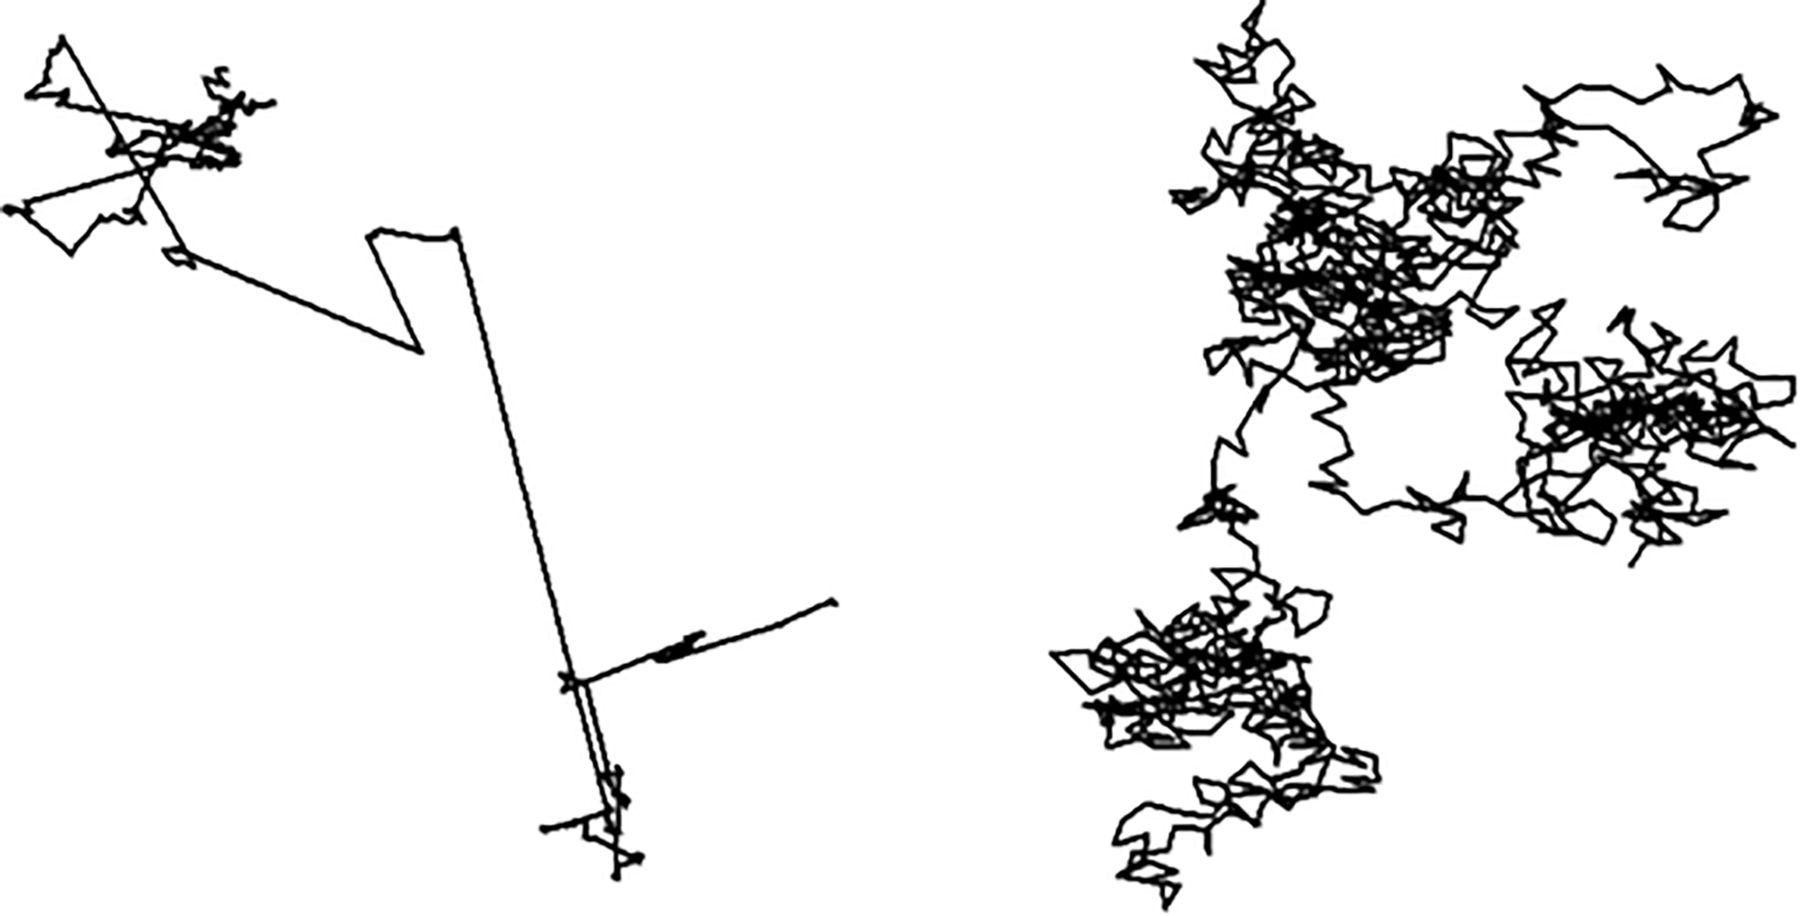
\includegraphics[width=0.8\linewidth]{gfx/levy-vs-brown}
 \caption[Lévy vs. Brownian walk]{An example of a Lévy walk (left) and a Brownian walk (right). The Lévy walk is dominated by the longest steps, whereas the Brownian walk is dominated by the most common step \cite{reynolds:2018}.}\label{fig:levy-vs-brown}
\end{figure}

The walk is scale invariant and forms fractal patterns. In this, one can also find the main idea and the original reasoning of why the Lévy walk has been associated with animal foraging behavior: after one territory has been explored for food, the animal then moves for a longer time in a random direction to find a new territory that has not been explored yet.

\subsection{Intermittent search}\label{ssec:intermittent-search}
The \textit{intermittent search} is closely related to the saltatory motion of animals that we have mentioned in \autoref{sec:MotAndExa}. The model includes two phases -- characterized by the mean time spent in them -- between which the searcher switches stochastically.

The first phase is the \textit{scanning} phase, in which the searcher is able to detect the target in its immediate vicinity. During the scanning phase the searcher is considered to move slowly and thus it is modeled as a diffusive motion with diffusion coefficient $D$.

The second phase is the \textit{motion} phase, in which the searcher moves rapidly and is unable to detect the target. This phase is usually modeled as ballistic motion with constant velocity $V$.

\begin{figure}[bth]
 \myfloatalign
 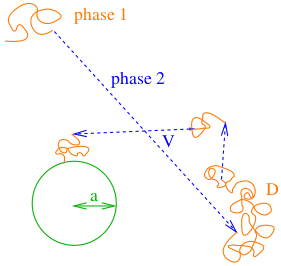
\includegraphics[width=0.4\linewidth]{gfx/intermittent-search}
 \caption[Abstract intermittent search]{Abstract of the intermittent search model. The searcher stochastically switches between a scanning phase (orange) and a motion phase (blue). The target vicinity is depicted by the green circle \cite{benichou:2011}.}\label{fig:intermittent-search}
\end{figure}

The intermittent search serves as an alternative to the previously mentioned Lévy walk and can be advantageous under certain conditions \cite{benichou:2011}.

\subsection{Sources of complexity in real systems}
The many different models for motion patterns or search strategies already give numerous parameters to consider, such as \eg the step length or velocity distribution, the persistency, and the mean time spent in different phases. Besides that, in real systems there are many more parameters that influence the efficiency of a search strategy: the size of the search realm, the size of the target or equivalently the detection range of the searcher, information contained in the environment, obstacles in the environment, crowded environments, the number of targets and searchers, interactions between targets and/or searchers, and many more factors need to be considered when one aims to create an adequate model. With all these things in mind, we overview a minimal model in the next section, which leads to interesting results, although all additional complexity is omitted.

\section{First-passage times of persistent random walkers}
Let us consider a model based on the two-dimensional \ac{prw} on a lattice in discrete time introduced in \autoref{ssec:2d-lattice} (see \autoref{fig:prw-lattice})\graffito{\textbf{Note:} The unit length of the problem is defined by the step size, lattice grid size, or target size, which are all set to $1$.}. Specifically, we want to look at bounded cubic domains of dimension $\Omega = [0,X)^2 \subset \N^2$, where only one target site is located at $\bv{n}_\textrm{tar}$. Furthermore, we assume periodic boundary conditions and $X \gg 1$, \ie the length of the lattice is much larger than the step size.

\begin{figure}[bth]
 \myfloatalign
 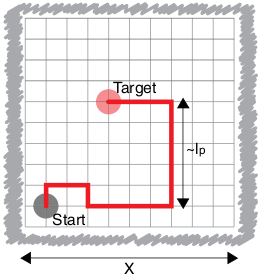
\includegraphics[width=0.4\linewidth]{gfx/prw-lattice}
 \caption[Persistent random walk on a lattice]{A persistent random walker on a cubic lattice, where one target site is located. The red line represents an example search trajectory \cite{tejedor:2012}.}\label{fig:prw-lattice}
\end{figure}

This situation is suitable for both biologically meaningful situations of a single target centered in a finite domain, and of homogeneously distributed targets in an infinite domain with density $1/V$, where \mbox{$V = X^2$} is the volume of the domain.

For simplicity, we set the turning probabilities $p_b = p_l = p_r \equiv q$, such that
\begin{equation*}
 q = \frac{1-p}{3},
\end{equation*}
\ie all possibilities that change the direction of motion are equally probable. We can furthermore write the probability of having $l$ consecutive steps in the same direction as
\begin{equation*}
 P(l) = (1-p) p^{l-1},
\end{equation*}
and we define the persistence length of the walk as
\begin{equation*}
 l_\textrm{p} = \avg{l} = \sum\limits_{l=1}^\infty l P(l) = \frac{1}{1-p},
\end{equation*}
which we will use as a defining parameter.

Following \cite{tejedor:2012}, we want to analyze the dependence of the \ac{mfpt} $\mfpt[\mean{\tau}]$ to the target site $\bv{n}_\textrm{tar}$ -- averaged over all possible starting positions and velocities -- on the persistence length $l_\textrm{p}$ and the lattice size $X$.

Consider a random searcher starting from $\bv{n}$ with initial velocity $\bv{e}_i$, where $\{\bv{e}_1, \bv{e}_2\}$ defines a basis of the lattice. Similar to \autoref{ssec:intApproach}, we can write an exact backward equation for the \ac{mfpt} $\mfpt[\tau(\bv{n},\bv{e}_i)]$ to the target $\bv{n}_\textrm{tar}$:
\begin{equation}\label{eq:tejedor-backward-equation}
 \begin{aligned}
  \mfpt[\tau(\bv{n},\bv{e}_i)] &= p \mfpt[\tau(\bv{n} + \bv{e}_i,\bv{e}_i)] + q \{ \mfpt[\tau(\bv{n} - \bv{e}_i,-\bv{e}_i)] + \mfpt[\tau(\bv{n} + \bv{e}_j,\bv{e}_j)] 
  \\
  &+ \mfpt[\tau(\bv{n} - \bv{e}_j,-\bv{e}_j)] \} + 1,
 \end{aligned}
\end{equation}
where $j \neq i \in \{1,2\}$. With the help of the Fourier transform,
\begin{equation*}
 \fourier{f}(\bv{q}) = \sum\limits_{\bv{n} \in \Omega} f(\bv{n}) \exp{(-i \bv{q} \cdot \bv{n})},
\end{equation*}
of a function $f(\bv{n})$, where $q_i = 2\pi k_i / X$ with $k_i \in [0, X)$, \autoref{eq:tejedor-backward-equation} can be solved explicitly. One can then average over all possible starting positions and velocities to obtain the final result \cite{tejedor:2012}:
\begin{equation}\label{eq:tejedor-exact-mfpt}
 \mfpt[\mean{\tau}] = \frac{-\epsilon(X^2 - 1)}{1 - \epsilon} + \frac{1+\epsilon^2}{1-\epsilon^2} \sum\limits_{\bv{q} \neq \bv{0}} \frac{1}{1 - h(\bv{q}, \epsilon)},
\end{equation}
where we introduced $\epsilon = p-q$ and
\begin{equation*}
 h(\bv{q},\epsilon) = \frac{(\epsilon -1)^2}{2} \sum\limits_{i=1}^2\frac{\cos{(\bv{q}\cdot\bv{e}_i)}}{1+ \epsilon^2 - 2\epsilon\cos{(\bv{q}\cdot\bv{e}_i)}}.
\end{equation*}
\autoref{eq:tejedor-exact-mfpt} is an exact expression for the search time of a persistent random searcher in dependence on the parameter $\epsilon$. We identify
\begin{equation*}
 l_\textrm{p} = \frac{1}{1-p} = \frac{4}{3} \frac{1}{1-\epsilon},
\end{equation*}
to emphasize that $\epsilon$ and the persistence length $l_\textrm{p}$ can be considered equivalently. The result can be seen in \autoref{fig:tejedor-graph}.

\begin{figure}[bth]
 \myfloatalign
 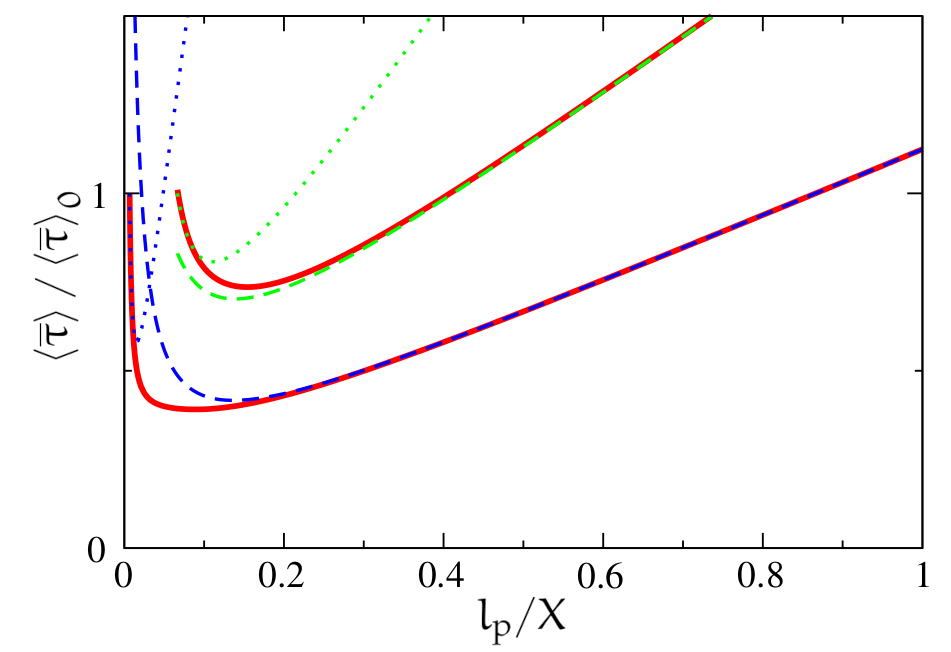
\includegraphics[width=0.8\linewidth]{gfx/tejedor-graph}
 \caption[]{\ac{mfpt} $\mfpt[\mean{\tau}]$ for a two-dimensional persistent random walker normalized by the \ac{mfpt} $\mfpt[\mean{\tau}]_0$ for a diffusive random walker in dependence on the persistence length $l_\textrm{p}$ normalized by the system size $X$, for $X = 10$ (upper set of curves) and $X = 100$ (lower set of curves) with exact results (red lines), approximation $\epsilon \ll 1$ (dotted lines) and $\epsilon \rightarrow 1$ (dashed lines) \cite{tejedor:2012}.}\label{fig:tejedor-graph}
\end{figure}

Let's take a look at two approximations made in \cite{tejedor:2012}. In the first case $\epsilon \ll 1$ is small and therefore $l_\textrm{p} \approx 4/3$, \ie the persistence length is comparable to the target size. For $\epsilon = 0$ we obtain a \ac{srw} as all directions become equally probable and we denote the search time of such a diffusive searcher by $\mfpt[\mean{\tau}]_0$. The \ac{mfpt} in the regime $\epsilon \ll 1$ then reads \cite{tejedor:2012}
\begin{equation} \label{eq:tejedor-approx1}
 \mfpt[\mean{\tau}] = A(\epsilon, V) (V - 1) + \frac{1}{D(\epsilon)} \mfpt[\mean{\tau}]_0,
\end{equation}
where $D(\epsilon) = \frac{1-\epsilon}{1+\epsilon}$ is the normalized diffusion coefficient of the persistent random walk and $A(\epsilon, V) = [B(V)-1]\epsilon + \mathcal{O}[\epsilon^2]$ is a nontrivial additive correction to the search time of a diffusive walker with
\begin{equation*}
 B(V) = \frac{2}{V}\sum\limits_{\bv{q}\neq0} \dfrac{\frac{1}{2} \sum\limits_{i=1}^2 [1-\cos(2\pi\bv{q}\cdot\bv{e}_i)]^2}{\left[\frac{1}{2} \sum\limits_{i=1}^2 1-\cos(2\pi\bv{q}\cdot\bv{e}_i)\right]^2}.
\end{equation*}
The approximation \ref{eq:tejedor-approx1} is accurate for small persistence lengths $l_\textrm{p}$ as can be seen in \autoref{fig:tejedor-graph}.

In the opposite case of $\epsilon \rightarrow 1$ the persistence length $l_\textrm{p} \rightarrow \infty$ becomes large and diverges. In this regime the \ac{mfpt} reads \cite{tejedor:2012}
\begin{equation*}
 \mfpt[\mean{\tau}] = \frac{2(X-1)}{1-\epsilon} + \frac{(X-1)^2}{2} + (1-\epsilon)\frac{(X-1)(X-2)(X+3)}{12} + \mathcal{O}[(1-\epsilon)^2],
\end{equation*}
which is accurate as long as $l_\textrm{p} \gg 1$ (see \autoref{fig:tejedor-graph}). Obviously, the mean search time becomes infinitely large for $\epsilon = 1$. This can be understood as follows: the persistency is $p = (3\epsilon + 1) / 4$ and therefore, for $\epsilon = 1$ the walker never changes its direction and gets stuck in infinitely long straight trajectories. As $\epsilon$ approaches $1$ also the probability of getting trapped in such long unsuccessful ballistic excursions becomes larger and therefore the search time increases.

\begin{figure}[bth]
 \myfloatalign
 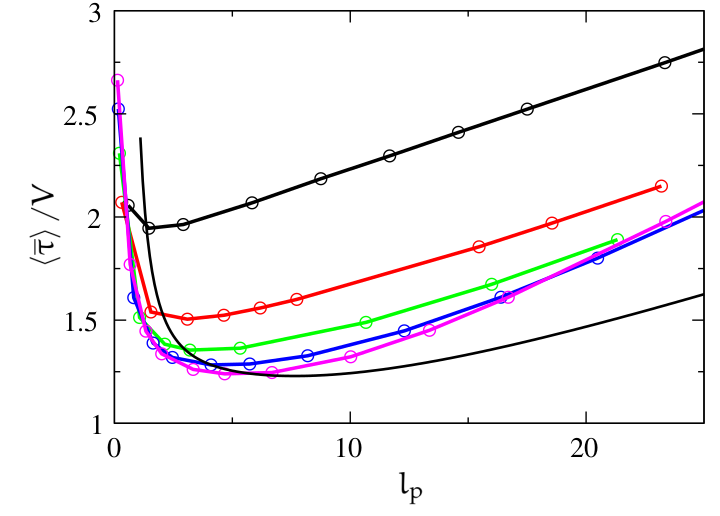
\includegraphics[width=0.8\linewidth]{gfx/tejedor-levy}
 \caption[]{Numerical simulation of the \ac{mfpt} for Lévy walks (lines with circles) and a persistent random walk (black line) on a two-dimensional lattice of size $X=50$. The plots with circles belong to Lévy walks with the parameters (from top to bottom): $\mu = 1.2, 1.4, 1.6, 1.8$, and $2$ \cite{tejedor:2012}.}\label{fig:tejedor-levy}
\end{figure}

Nevertheless, the minimum of the \ac{mfpt} $\mfpt[\mean{\tau}]$ in dependence on the persistence length $l_\textrm{p}$ can be found by analyzing the exact result from \autoref{eq:tejedor-exact-mfpt} (see \autoref{fig:tejedor-graph}). It appears that the persistence length needs to be of the same order of magnitude as the system size in order to minimize the average search time \cite{tejedor:2012}. For $l_\textrm{p} \ll X$, the search has diffusive properties and therefore is inefficient, whereas for $l_\textrm{p} \gg X$ the walker is likely to get trapped in long unsuccessful straight runs. Thus, one would expect the optimal persistence length to be in the regime $l_\textrm{p} \propto X$.

As a last point, we want to briefly compare the performance of the persistent random walk to the Lévy walk strategy as it has been presented in \autoref{ssec:levy-walk}. From \autoref{fig:tejedor-levy} we see that the persistent random walk strategy leads to a minimum in the search time that is smaller than any minimum in the search times for the Lévy strategies. Only for the parameter $\mu = 2$ -- for which the distribution of the lengths of ballistic excursions has a finite second moment and thus is no longer of the Lévy type -- the Lévy walk can compete with the persistent random walk in the given scenario. Therefore, \citeauthor{tejedor:2012} \cite{tejedor:2012} conclude that the persistent random walk, as introduced above, performs better than any Lévy walk in the biologically relevant cases of either a single target or patterns of targets characterized by a peaked distribution of target to target distance.

%*****************************************
%*****************************************
%*****************************************
%*****************************************
%*****************************************
